\section{Method}

In this section we discuss the way in which we process and analyse the data we obtain from EUMETSAT. First we detail the process of thresholding, which we use to distinguish between cloud and land pixels. Then, we explain how these thresholds are used to calculate cloud coverage and

\subsection{Thresholding}
% part about skewing unnecessary?
The most essential part of processing the EUMETSAT images is the ability to
differentiate between cloud and land. Clouds have a much higher reflectance than
land -- if mistakenly identified as land pixels, they will erroneously skew the
value of those pixels to higher values. However we can exploit the fact that
clouds have a much higher reflectance than areas of land (notable
  exceptions to this are snow, ice and salt pans) in order to differentiate
them. It follows that the distribution of values for a single pixel over a large
enough number of days will be bimodal, the peak at the smaller value
corresponding to land pixels and the peak at the larger value corresponding to
cloudy pixels. The task is now one of producing thresholds that reliably
separate the two peaks. Otsu's method \citep{gonzalez2008} separates pixels into
two groups, or \emph{classes}, by maximising the variance between these classes,
making it an optimum method for thresholding \footnote{We have made use of
  \texttt{scipy}'s Otsu thresholding implementation.}. An example of Otsu
thresholding at work is shown in Figure \ref{fig:otsu} for a random pixel.
\begin{figure}
  \centering
    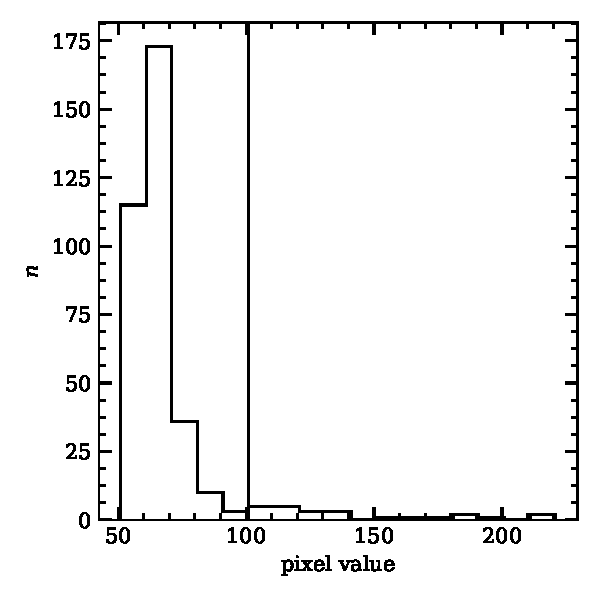
\includegraphics[width=\linewidth]{figures/otsu_bimodal.pdf}
    \caption{The histogram of pixel values for a random pixel. Shown
      by the vertical line is the threshold calculated using Otsu's method -- it can
      be seen how well this method separates the two peaks.}
    \label{fig:otsu}
\end{figure}
All pixels with a value below the threshold will be identified as land and all
pixels with a value greater than or eequal to the threshold will be identified
as cloud. Now that we have the method for calculating the threshold of a single
pixel all that remains is to apply it to the entire image, the process for doing
so is detailed in Figure \ref{fig:thr_fc}.
\begin{figure}[t!]
  \centering
  \includegraphics{threshold_flowchart.pdf}
  \caption{Flowchart for calculating threshold values.}
  \label{fig:thr_fc}
\end{figure}

\subsection{Cloud coverage}
Using the thresholds calculated by the method in Figure \ref{fig:thr_fc} we
produce daily cloud masks, which are arrays of the same size as the input image
containing with values of 1 for cloud pixels and 0 for land pixels. The number
of cloud pixels $n_{\mathrm{cloud}}$ for a given day, then, are found by summing
the cloud mask. Cloud coverage is calculated as the ratio of cloud pixels to
total land pixels in the image $N$
\begin{equation}
  \mathrm{CF} = \frac{n_{\mathrm{cloud}}}{N} \,,
  \label{eq:cloud_frac}
\end{equation}
where $N$ is found by summing over all of the land pixels in the land mask for
the given region.

\subsection{NDVI}
%% Local Variables:
%% fill-column: 80
%% End:
